%!TeX root = Chapter_Method
\documentclass[../../CompleteThesis/Complete_1stDraft.tex]{subfiles}
\begin{document}
	
	\section[First $\sigma$ estimate]{Estimating $\sigma$ from Data: First Estimate}
	\label{Sec:Method_FirstSigmaEstimate}
	This section contains a walk through of the method to back diffuse a given ice core depth series to attempt to restore as much of the original signal as possible. For now, the method has been developed for sections that has been dated to be between the two volcanic eruptions Laki and Tambora, as these are very well dated, and thus it is possible to find the optimal diffusion length to back diffuse with as the actual number of annual layers is exactly known for this data series. The method is easily modified for any other dated depth series, as what is needed is just the number of annual layers in the given data series.\\
	Figures \ref{Fig:FlowchartOptimalDiffLen} and \ref{Fig:FlowchartBackDiffusion} show a flowchart of the method used to estimate the diffusion length of a depth series with a preliminary guess of number of annual layers. In the following sections each of the steps in the method will be discussed more thoroughly and examples will be given, all based on the Greenlandic ice core drilled at Site A near Crete(REFERENCES!!!).
	The method is built such that it takes two inputs - the isotopic depth series, and the specifications for the particular ice core - and uses these for the first preliminary computations needed to make a first, naïve guess of the diffusion length, $\sigma_0$.
	This diffusion length is then used to deconvolute the data and give a first estimate of the number of peaks in the data series. If this number is different from the already specified number of annual layers - in this case 32 - then the diffusion length will be updated accordingly: If the counted number is higher(lower) than the actual number, the diffusion length is adjusted downwards(upwards) with $\Delta\sigma_2$ and the deconvolution and peak counting is performed again.
	On the other hand, if the counted number is equal to the actual number, then the diffusion length is optimized to find the largest diffusion length which still gives the actual number of counted peaks. When this $\sigma_{\text{final}}$ is reached, the algorithm stops and returns the final diffusion length estimate along with the associated back diffused depth series.
	\begin{figure}
		\begin{tikzpicture}[node distance=1.5cm, auto]
			\node(start) [startstop] {START};
			%----------------------------------------------------%
			\node(in1) [io, left of=start, xshift=-2.5cm] {Depth series};
			\node(empty1) [below of=in1, yshift=0.12cm] {};
			\node(empty2) [below of=in1, xshift=-0.15cm] {};
			%		\node(in1pro1) [process, below of=in1, yshift=-0.5cm] {Spline interpolation};
			\node(in1pro2) [process, below of=in1, yshift=-2cm] {Spectral analysis};
			\node(decSpec1) [decision, below of=in1pro2, scale = 0.8, align=center] {DCT ?\\(Interpolation)};
			\node(decSpec2) [decision, left of=decSpec1, scale=0.8, xshift = -1.2cm, align=center] {FFT ?\\(Interpolation)};
			\node(decSpec3) [decision, right of=decSpec1, scale=0.8, xshift = 0.8cm] {NDCT ?};
			
			\node(in1pro3) [process, below of=decSpec1] {Wiener filter};
			
			\draw[arrow] (in1) -- (start);
			\draw[-] (start) |- (empty2);
			\draw[arrow] (empty1) -- (in1pro2);
			%		\draw[arrow] (in1pro1) -- (in1pro2);
			\draw[arrow] (in1pro2) -- (decSpec1);
			\draw[arrow] (in1pro2) -- (decSpec2);
			\draw[arrow] (in1pro2) -- (decSpec3);
			\draw[arrow] (decSpec1) -- (in1pro3);
			\draw[arrow] (decSpec2) -- (in1pro3);
			\draw[arrow] (decSpec3) -- (in1pro3);
			%	\draw[arrow] (in1pro3) -- (in1pro4);
			
			%----------------------------------------------------%
			
			\node(in2) [io, right of=start, xshift=2.5cm] {Core specs};
			\node(in2pro1) [process, below of=in2, yshift=-0.5cm] {Density profile};
			\node(in2pro2) [process, below of=in2pro1] {Diffusion profile};
			\node(in2pro3) [process, below of=in2pro2] {$\sigma_0$\textbf{ estimate}};
			\node(decSigma1) [decision, below of=in2pro3, scale = 0.8] {$\sigma_0 = \sigma_{\text{const}}$?};
			\node(decSigma2) [decision, right of=decSigma1, scale = 0.8, xshift=0.8cm] {$\sigma_0 = \sigma(z)$?};
			\node(decSigma3) [decision, left of=decSigma1, scale = 0.8, xshift=-0.8cm] {$\sigma_0 = \sigma_{\text{input}}$?};
			
			
			\draw[arrow] (in2) -- (start);
			\draw[arrow] (start) |- (in2pro1);
			\draw[arrow] (in2pro1) -- (in2pro2);
			\draw[arrow] (in2pro2) -- (in2pro3);
			\draw[arrow] (in2pro3) -- (decSigma1);
			\draw[arrow] (in2pro3) -- (decSigma2);
			\draw[arrow] (in2pro3) -- (decSigma3);
			
			%----------------------------------------------------%
			\node(pro0) [process, below of=start, yshift=-6.5cm] {Frequency Filters};
			\node(pro1) [process, below of=pro0,align=center] {\textbf{Deconvolution}\\(Uniform resampling)};
			\node(stop) [startstop, below of=pro1] {\textbf{STOP}};
			\node(out1) [io, right of=stop, align=center, xshift=2.2cm, text width=2.5cm] {\footnotesize{Back diffused depth series}};
			\node(out2) [io, below of=out1, align=center] {\footnotesize{$\sigma_{\text{out}}$}};
			\draw[arrow] (in1pro3) |- (pro0);
			\draw[arrow] (decSigma1) |- (pro0);
			\draw[arrow] (decSigma2) |- (pro0);
			\draw[arrow] (decSigma3) |- (pro0);
			\draw[arrow] (pro0) -- (pro1);
			\draw[arrow] (pro1) -- (stop);
			\draw[arrow] (stop) -- (out1);
			\draw[arrow] (stop) |- (out2);
			
			%		\draw[arrow] (in2pro3) -| (pro0);
			
		\end{tikzpicture}
		\caption[Flowchart]{Flowchart of initialization method for back diffusion of a depth series given a diffusion length estimate.}
		\label{Fig:FlowchartBackDiffusion}
	\end{figure}	
	
	
	\begin{figure}
		\begin{tikzpicture}[node distance=1.5cm, auto]
			
			\node(pro0) [process] {Frequency Filters};
			\node(pro1) [process, below of=pro0,align=center] {\textbf{Deconvolution}\\(Uniform resampling)};
			\node(pro2) [process, below of=pro1] {Count N Peaks};
			\node(dec1) [decision, below of=pro2, yshift=-.5cm] {$N = N_{\text{yrs}}$ ? };
			
			%		\draw[arrow] (in1pro3) -| (pro0);
			%		\draw[arrow] (in2pro3) -| (pro0);
			\draw[arrow] (pro0) -- (pro1);
			\draw[arrow] (pro1) -- (pro2);
			\draw[arrow] (pro2) -- (dec1);
			\draw[arrow] (-4,0) to (pro0);
			\draw[arrow] (4,0) to (pro0);
			%----------------------------------------------------%	
			\node(pro3a) [process, below of=dec1, xshift=-3cm] {$\sigma = \sigma + \Delta \sigma_1 $};
			\node(pro3apro1) [process, below of=pro3a,align=center] {\textbf{Deconvolution}\\(Uniform resampling)};
			\node(pro3apro2) [process, below of=pro3apro1]  {Count N peaks};
			\node(pro3apro3) [process, below of=pro3apro2, xshift=-2cm] {$\sigma_{\text{final}} = \sigma - 2\cdot\Delta\sigma_1$};
			\node(stop) [startstop, right of=pro3apro3, xshift=2.5cm] {STOP};
			\node(out1) [io, right of=stop, xshift=2.5cm, text width=2.5cm] {\footnotesize{Back diffused depth series}};
			\node(out2) [io, below of=out1, text width=1.1cm] {$\sigma_{\text{final}}$};
			
			
			\draw [arrow] (dec1) -| node[anchor=east] {yes} (pro3a);
			\draw [arrow] (pro3a) -- (pro3apro1);
			\draw [arrow] (pro3apro1) -- (pro3apro2);
			\draw [arrow] (pro3apro2) --++ (2,0) node [anchor=west] {If $N = N_{\text{yrs}}$} |- (pro3a);		
			\draw[arrow] (pro3apro2) --++ (-2,0) node [anchor=east] {If $N > N_{\text{yrs}}$} -| (pro3apro3);
			\draw[arrow] (pro3apro3) -- (stop);
			\draw[arrow] (stop) -- (out1);
			\draw[arrow] (stop) |- (out2);
			
			%----------------------------------------------------%	
			\node(pro3b1) [process, right of=dec1, xshift=3.2cm] {$\sigma = \sigma - \Delta\sigma_2$};
			\node(pro3b2) [process, below of=dec1, xshift=4.7cm] {$\sigma=\sigma+\Delta\sigma_2$};
			
			
			\draw [arrow] (dec1) --(2.2,-5) node[anchor=south] {$N > N_{\text{yrs}}$} -- (pro3b1);
			\draw[arrow] (dec1) -- (0,-6.5) node[anchor=north] {$N < N_{\text{yrs}}$} -- (pro3b2);
			\draw[arrow] (pro3b1) |- (pro1);
			\draw[arrow] (pro3b2) --++ (2,0) |- (pro1);		
			
		\end{tikzpicture}
		\caption[Flowchart]{Flowchart of method for optimal diffusion length computation.}
		\label{Fig:FlowchartOptimalDiffLen}
	\end{figure}
	
	%\begin{figure}
	%	\begin{tikzpicture}[node distance=1.5cm, auto]
	%		\node(start) [startstop] {START};
	%		%----------------------------------------------------%
	%		\node(in1) [io, left of=start, xshift=-3.5cm] {Depth series};
	%		\node(in1pro1) [process, below of=in1, yshift=-0.5cm] {Spline interpolation};
	%		\node(in1pro2) [process, below of=in1pro1] {Spectral analysis};
	%		\node(in1pro3) [process, below of=in1pro2] {Wiener filter};
	%		%	\node(in1pro4) [process, below of=in1pro3] {\textbf{Frequency filters}};	
	%		
	%		\draw[arrow] (in1) -- (start);
	%		\draw[arrow] (start) |- (in1pro1);
	%		\draw[arrow] (in1pro1) -- (in1pro2);
	%		\draw[arrow] (in1pro2) -- (in1pro3);
	%		%	\draw[arrow] (in1pro3) -- (in1pro4);
	%		
	%		%----------------------------------------------------%
	%		\node(in2) [io, right of=start, xshift=3.5cm] {Core specs};
	%		\node(in2pro1) [process, below of=in2, yshift=-0.5cm] {Density profile};
	%		\node(in2pro2) [process, below of=in2pro1] {Diffusion profile};
	%		\node(in2pro3) [process, below of=in2pro2] {$\sigma_0$\textbf{ estimate}};
	%		
	%		\draw[arrow] (in2) -- (start);
	%		\draw[arrow] (start) |- (in2pro1);
	%		\draw[arrow] (in2pro1) -- (in2pro2);
	%		\draw[arrow] (in2pro2) -- (in2pro3);
	%		
	%		%----------------------------------------------------%
	%		\node(pro0) [process, below of=start, yshift=-4.5cm] {\textbf{Frequency Filters}};
	%		\node(pro1) [process, below of=pro0] {\large{\textbf{BACK DIFFUSE}}};
	%		\node(pro2) [process, below of=pro1] {Count N Peaks};
	%		\node(dec1) [decision, below of=pro2, yshift=-.5cm] {$N = 32$ ? };
	%		
	%		\draw[arrow] (in1pro3) -| (pro0);
	%		\draw[arrow] (in2pro3) -| (pro0);
	%		\draw[arrow] (pro0) -- (pro1);
	%		\draw[arrow] (pro1) -- (pro2);
	%		\draw[arrow] (pro2) -- (dec1);
	%		
	%		%----------------------------------------------------%	
	%		\node(pro3a) [process, below of=dec1, xshift=-3cm] {$\sigma = \sigma + \Delta \sigma_1 $};
	%		\node(pro3apro1) [process, below of=pro3a] {Back diffuse};
	%		\node(pro3apro2) [process, below of=pro3apro1]  {Count N peaks};
	%		\node(pro3apro3) [process, below of=pro3apro2, xshift=-2cm] {$\sigma_{\text{final}} = \sigma - 2\cdot\Delta\sigma_1$};
	%		\node(stop) [startstop, right of=pro3apro3, xshift=2.5cm] {STOP};
	%		\node(out1) [io, right of=stop, xshift=2.5cm, text width=2.5cm] {\footnotesize{back diffused depth series}};
	%		\node(out2) [io, below of=out1, text width=1.1cm] {$\sigma_{\text{final}}$};
	%		
	%		
	%		\draw [arrow] (dec1) -| node[anchor=east] {yes} (pro3a);
	%		\draw [arrow] (pro3a) -- (pro3apro1);
	%		\draw [arrow] (pro3apro1) -- (pro3apro2);
	%		\draw [arrow] (pro3apro2) --++ (2,0) node [anchor=west] {If $N$ = 32} |- (pro3a);		
	%		\draw[arrow] (pro3apro2) --++ (-2,0) node [anchor=east] {If $N > $  32} -| (pro3apro3);
	%		\draw[arrow] (pro3apro3) -- (stop);
	%		\draw[arrow] (stop) -- (out1);
	%		\draw[arrow] (stop) |- (out2);
	%		
	%		%----------------------------------------------------%	
	%		\node(pro3b1) [process, right of=dec1, xshift=3.2cm] {$\sigma = \sigma - \Delta\sigma_2$};
	%		\node(pro3b2) [process, below of=dec1, xshift=4.7cm] {$\sigma=\sigma+\Delta\sigma_2$};
	%		
	%		
	%		\draw [arrow] (dec1) --(2.45,-11) node[anchor=south] {$N > 32$} -- (pro3b1);
	%		\draw[arrow] (dec1) -- (0,-12.5) node[anchor=north] {$N < 32$} -- (pro3b2);
	%		\draw[arrow] (pro3b1) |- (pro1);
	%		\draw [arrow] (pro3b2) --++ (2,0) |- (pro1);		
	%		
	%	\end{tikzpicture}
	%	\caption[Flowchart]{Flowchart of method for diffusion length computation.}
	%	\label{Fig:FlowchartDiffLen}
	%\end{figure}	
	
	
	
	
	\subsection[Input]{Input}
	\label{Subsec:Method_FirstSigmaEstimate_Input}
	To compute the final diffusion length and depth series, two inputs are needed: the measured isotopic depth series and the specifications of the examined core. Through this section all examples have been carried out using the core Site A.\\
	\begin{figure}
		\centering
		\includegraphics[width=0.9\textwidth]{SiteA_d18OInsert.jpg}
		\caption[Full $\delta^{18}$O record with insert, Site A]{The entire ice core isotopic profile from Site A, with a zoom in on the estimated depth series spanning from Tambora to Laki.}
		\label{fig:SiteA_d18OInsert}
	\end{figure}
	
	
	\begin{table}[ht]
		\centering
		\begin{adjustbox}{width=1.4\textwidth,center=\textwidth}
			
			\begin{tabular}{l*{10}{c}}
				
				\toprule
				Core &  Drilled &  Core length &    \multicolumn{2}{c}{Geographic position}		&  Elevation &   Laki &  Tambora &  Mean accum. rate &  Temp. at 10m &   Temp at 20m \\ \cmidrule{4-5}
				&&&   Latitude &  Longitude &&&&&&\\
				ID & [Yr] & [m] & [\degree N] & [\degree E] & [m a.s.l.] & [m] & [m] & [m ice/Yr] &[\degree C]&[\degree C]\\
				\midrule
				Crete &     1974 &       404.0 &  71.12 &  322.68 &  3172 &  74.75 &  64.70 &   0.280 & -30.40 & -30.16 \\
				Milcent &     1973 &       398.0 &  70.30 &  315.00 &  2410 &        &        &   0.530 & -22.30 &  -0.00 \\
				Camp C &     1977 &       100.1 &  77.18 &  298.89 &  1880 &  91.50 &  78.50 &   0.380 & -24.29 & -24.35 \\
				SiteA &     1985 &       128.6 &  70.63 &  324.18 &  3092 &  80.85 &  70.90 &   0.307 & -29.41 & -29.41 \\
				SiteB &     1984 &       105.6 &  70.65 &  322.52 &  3138 &  83.70 &  73.00 &   0.327 & -29.77 & -29.48 \\
				SiteC &     1984 &        24.9 &  70.68 &  321.21 &  3072 &        &        &   0.340 & -29.10 & -28.54 \\
				SiteD &     1984 &       100.1 &  70.64 &  320.38 &  3018 &  93.80 &  81.50 &   0.365 & -28.30 & -27.89 \\
				SiteE &     1985 &        77.8 &  71.76 &  324.15 &  3087 &  62.95 &  53.40 &   0.225 & -30.37 & -30.41 \\
				SiteF &     1985 &        25.7 &  71.49 &  324.12 &  3092 &        &        &   0.237 & -30.42 & -30.36 \\
				SiteG &     1985 &        70.8 &  71.15 &  324.16 &  3098 &  69.40 &  60.50 &   0.251 & -30.10 & -30.01 \\
				SiteH &     1985 &        26.2 &  70.87 &  324.16 &  3102 &        &        &   0.277 & -29.59 & -29.53 \\
				\bottomrule
			\end{tabular}
		\end{adjustbox}
		\label{tab:CoreSpecs}
		\caption[Ice core Specs]{Overview of specifications of all examined Greenlandic ice cores.}
	\end{table}
	
	In Figure \ref{fig:SiteA_d18OInsert} the depth series between the eruptions Laki and Tambora can be seen along with the entire ice core in the background. This is the diffused, measured raw data from Site A. Dating of the ice cores has been carried out by matching Electrical Conductivity Measurements (ECM, Section \ref{Sec:??}) with water isotopic - in this case $\delta^{18}$O - data measured at the same depths. By doing so it is possible to identify known volcanic horizons in the ECM data and thus getting a sharp marker of when the precipitation of that given depth fell. In Figure \ref{fig:SiteA_ECMd18O_combo} the matched ECM and $\delta^{18}$O profiles can be seen with Tambora marked at depth \_\_\_\_ and Laki at depth \_\_\_\_.
	
	\begin{figure}[h]
		\centering
		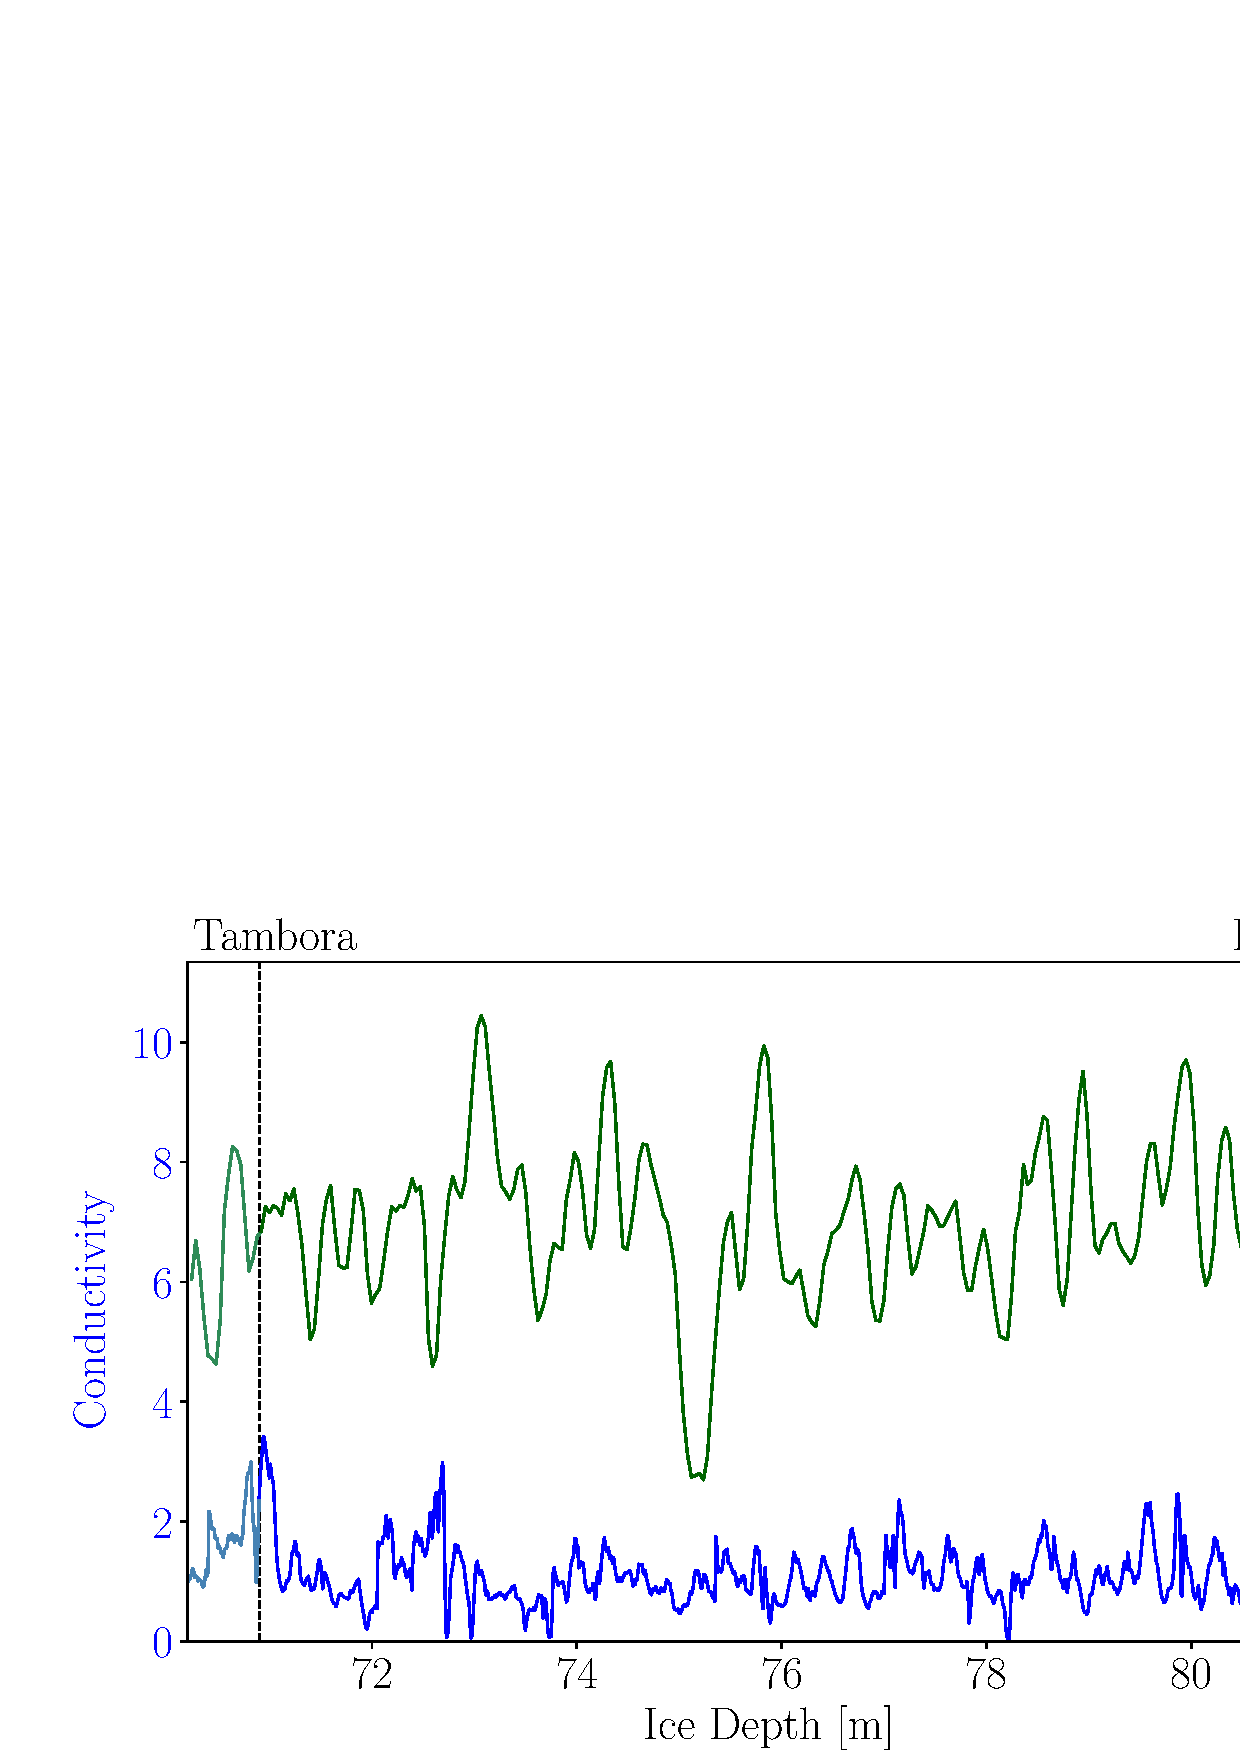
\includegraphics[width=0.7\textwidth]{SiteA_ECMd18O_combo.jpg}
		\caption[ECM and d18O data at LT, Site A.]{Two depth profiles from the core drilled at Site A showing accordingly the measured $\delta^{18}$O isotopic values and the conductivity measurements in the depth ranging from the estimated Tambora eruption to the Laki eruption.}	
		\label{fig:SiteA_ECMd18O_combo}
	\end{figure}
	\subsection[Preliminary Computations]{Preliminary Computations}
	\label{Subsec:Method_FirstSigmaEstimate_PrelimComputations}
	From the inputs a number of preliminary computations need to be carried out before the optimization of the diffusion length can be performed. For the depth series this consists of first interolating the data to make sure that the depth series is evenly sampled, then an analysis of signal and noise in the frequency spectrum needs to be carried out, and from this spectral analysis a Wiener filter can be constructed to find the optimal high frequency cut off, where as much noise as possible is filtered away while losing as little of the signal as possible. These computations are all based on the depth series data and use only signal analysis theory.\\
	The input of core specifications on the other hand is used to give a more theoretical view of the situation. From these preliminary inputs, containing accumulation rate, borehole temperatures, altitudes and other conditions, it is possible to use ice core and ice flow theory to compute initial estimates of density and diffusion profiles at the given site. From these profiles along with the volcanic horizons indicating the series of interest, an initial estimate of the diffusion length at the depth of Laki to Tambora.\\
	Firstly, the computations associated with the core site specifications are considered and later the ones associated with inputted depth series are described. 
	
	
	
	
	\subsubsection[Density Profile]{Core Specifications: Density Profile}
	\label{Subsubsec:Method_FirstSigmaEstimate_PrelimComputations_DensProfile}
	\marginnote{%
		\footnotesize
		\centering
		\begin{tabular}{lc}
			\toprule
			Variable & Default\\
			\midrule
			$T_0$ & (218.15 K)  \\
			$\dot{b}_0$ & (0.027 $\frac{\text{m}}{\text{yr}}$) \\
			$\rho_{\text{surf}}$ & (330 $\frac{\text{kg}}{\text{m}^3}$) \\
			$\rho_{\text{ice}}$ & 917 $\frac{\text{kg}}{\text{m}^3}$ \\
			$\rho_{\text{Cr}}$ & 550 $\frac{\text{kg}}{\text{m}^3}$ \\
			$\rho_{\text{CO}}$ & 804 $\frac{\text{kg}}{\text{m}^3}$ \\
			$f_0^{\text{init}}$ & 1 \\
			$f_1^{\text{init}}$ & 1 \\
			$z_{\text{meas}}$ & - \\
			$\rho_{\text{meas}}$ & - \\
			\bottomrule
		\end{tabular}
		\captionof{table}{\footnotesize Input variables and their default values.}
		\label{tab:DensInputVar}
	}[0.5cm]%
	From the input core specifications, specifically the surface temperature, $T_0$ and accumulation rate, $\dot{b}_0$, it is possible to estimate a density/depth profile through the Herron-Langway model described in section \ref{sec:Theory}. This section will contain a brief walk through of the algorithm used to estimate this profile.
	The Herron-Langway density profile program needs an estimate of surface temperature and annual accumulation rate, but does also take depth-density measurements into the calculations, if they exist and a surface density can also be specified to be taken into account. The adjustable input values and their default values can be seen in Table \ref{tab:DensInputVar}. The parameters describe surface temperature, $T_0$, annual accumulation rate, $\dot{b}_0$, surface density, $\rho_0$, density of ice, $\rho_{\text{ice}}$, critical density, $\rho_{\text{Cr}}$, close off density, $\rho_{\text{CO}}$, fit fudge parameters for upper and lower densification zones, $f_0$ and $f_1$, and depth and density measurements, $z_{\text{meas}}$ and $\rho_{\text{meas}}$. 
	
	The program is built to estimate a semi-analytical estimate of the depth-density profile given certain surface conditions. Furthermore it returns not only the density profile but computes the derivatives $\frac{d\rho}{dz}$ and $\frac{d\rho}{dt}$, and a timescale estimate for the profile. Two calculations repeats themselves, the computation of the values $k_0$ and $k_1$ and will just be mentioned this once:
	\begin{equation}
		k_0 = f_0\cdot 11\cdot e^{-\frac{10160}{T_0\cdot R}}
		\label{Eq:k0}
	\end{equation}
	\begin{equation}
		k_1 = f_1\cdot 575\cdot e^{-\frac{21400}{T_0\cdot R}}
		\label{Eq:k1}
	\end{equation}
	
	The program consists of the following different modules:
	\begin{itemize}
		\item \lstinline[columns=fixed]|calc_dens0|:  Calculate surface density. Use default surface value, $\rho_{\text{surf}} = 330 \frac{\text{kg}}{\text{m}^3}$, if no measurements available. Otherwise calculate surface density by using $z_{\text{init}} = z_{\text{meas}}$[0] and $\rho_{\text{init}} = \rho_{\text{meas}}$[0] as:
		\begin{equation}
			\rho_{\text{surf}} = \frac{\rho_{\text{ice}}}{1 + \frac{\rho_{\text{ice}} - \rho_{\text{init}}}{\rho_{\text{init}}}\cdot e^{z_{\text{init}}\cdot \rho_{\text{ice}}\cdot k_0}}
			\label{Eq:rhoSurf}
		\end{equation}
		
		\item \lstinline[columns=fixed]|calc_zCr|: Calculate ice depth of critical density (i. e. depth of boundary between first and second stage of densification), $\rho_{\text{Cr}}=550\frac{\text{kg}}{\text{m}^3}$:
		\begin{equation}
			z_{\text{Cr}} = \frac{1}{\rho_{\text{ice}}\cdot k_0}\cdot\left(\ln \left[\frac{\rho_{\text{Cr}}}{\rho_{\text{ice}} - \rho_{\text{Cr}}}\right]-\ln\left[\frac{\rho_{\text{surf}}}{\rho_{\text{ice}} - \rho_{\text{surf}}}\right]\right)
			\label{Eq:zCr}
		\end{equation}
		
		\item \lstinline[columns=fixed]|model_0|, \lstinline[columns=fixed]|model_1|: Models describing the two first stages of densification. Computed as:
		\begin{equation}
			\rho_0(z) = \rho_{\text{ice}}\cdot \left(\frac{Z_0(z)}{1+Z_0(z)}\right), \qquad Z_0(z) = e^{\rho_{\text{ice}}\cdot k_0 \cdot z + \ln(\frac{\rho_{\text{surf}}}{\rho_{\text{ice}} - \rho_{\text{surf}}})}
			\label{Eq:rhoModel0}
		\end{equation}
		\begin{equation}
			\rho_1(z) = \rho_{\text{ice}}\cdot \left(\frac{Z_1(z)}{1+Z_1(z)}\right), \qquad Z_1(z) = e^{\rho_{\text{ice}}\cdot k_1 \cdot \frac{z - z_{Cr}}{\sqrt{\dot{b}_0}} + \ln(\frac{\rho_{\text{Cr}}}{\rho_{\text{ice}} - \rho_{\text{Cr}}})}
			\label{Eq:rhoModel1}
		\end{equation}
		where $\rho_0(z)$ corresponds to all $z \leq z_{\text{Cr}}$ and $\rho_1(z)$ to all $z > z_{\text{Cr}}$.
		\item \lstinline[columns=fixed]|fit_f0|,  \lstinline[columns=fixed]|fit_f1|: Both modules are only used if any measured data is available. If depth and density data exists then these routines will compute the optimal (least-squares) fudge parameters $f_0$ and $f_1$, see Equations \ref{Eq:k0} and \ref{Eq:k1}, by fitting the data with the models for $\rho_0$ and $\rho_1$ described above. These updated fudge parameters are then henceforth used in the programs computations.
		
		\item \lstinline[columns=fixed]|dens_to_depth|: From a given density, calculate the corresponding depth. Same as \lstinline[columns=fixed]|calc_zCr|, but for any density, in both stages of densification.
		\begin{equation}
			z_0(\rho) = \frac{1}{\rho_{\text{ice}}\cdot k_0}\left(\ln\left[\frac{\rho}{\rho_{\text{ice}} - \rho}\right] - \ln\left[\frac{\rho_{\text{surf}}}{\rho_{\text{ice}} - \rho_{\text{surf}}}\right]\right), \qquad \rho \leq \rho_{\text{Cr}}
			\label{Eq:rhoToDepth_0}
		\end{equation}	
		\begin{equation}
			z_1(\rho) = \frac{\dot{b}_0}{\rho_{\text{ice}}\cdot k_1}\left(\ln\left[\frac{\rho}{\rho_{\text{ice}} - \rho}\right] - \ln\left[\frac{\rho_{\text{Cr}}}{\rho_{\text{ice}} - \rho_{\text{Cr}}}\right]\right) + z_{\text{Cr}}, \qquad \rho > \rho_{\text{Cr}}
			\label{Eq:rhoToDepth_1}
		\end{equation}		
		
		\item \lstinline[columns=fixed]|drho_dz_0|, \lstinline[columns=fixed]|drho_dz_1|: Compute the first derivative with respect to $z$, both stages of densification:
		\begin{equation}
			\frac{d\rho_0}{dz} = \rho_{\text{ice}}^2\cdot k_0 \cdot Z_0\cdot \left[\frac{1 + 2\cdot Z_0}{(1 + Z_0)^2}\right], \qquad \rho_0 \leq \rho_{\text{Cr}}
			\label{Eq:drho_dt_0}
		\end{equation}
		\begin{equation}
			\frac{d\rho_1}{dz} = \rho_{\text{ice}}^2\cdot k_1 \cdot Z_1\cdot \frac{1}{\sqrt{\dot{b}_0}}\cdot \left[\frac{1 + 2\cdot Z_1}{(1 + Z_1)^2}\right], \qquad \rho_0 > \rho_{\text{Cr}}
			\label{Eq:drho_dt_1}
		\end{equation}
		with $Z_0$ and $Z_1$ as described in Equations \ref{Eq:rhoModel0} and \ref{Eq:rhoModel1}.
		
		\item \lstinline[columns=fixed]|drho_dt|: Compute the time evolution of the density profile as the derivative of $\rho$:
		\begin{equation}
			\frac{d\rho_0}{dt} = k_0 \cdot\dot{b}_0\cdot (\rho_{\text{ice}} - \rho_{\text{surf}}), \qquad \rho_0 \leq \rho_{\text{Cr}}
		\end{equation}
		\begin{equation}
			\frac{d\rho_1}{dt} = k_1 \sqrt{\cdot\dot{b}_0}, \qquad \rho_1 > \rho_{\text{Cr}}
		\end{equation}	
		\item \lstinline[columns=fixed]|time_scale_HL|: From the best optimized Herron-Langway depth-density profile estimate it is possible to compute a age-density profile estimate for the firn column. For the first stage of densification this is computed as:
		\begin{equation}
			t_0(\rho) = \frac{1}{k_0 \dot{b}_0} \cdot \ln\left[\frac{\rho_{\text{ice}} - \rho_{\text{surf}}}{\rho_{\text{ice}} - \rho}\right], \qquad \rho_0 \leq \rho_{\text{Cr}}
		\end{equation}
		The age of the second stage of densification is computed in the same fashion, and then adding the age at the boundary between the two stages, that is, the critical density, $t_{\text{Cr}}$:
		\begin{equation}
			t_1(\rho) = \frac{1}{k_1 \sqrt{\dot{b}_0}}\cdot\ln\left[\frac{\rho_{\text{ice}} - \rho_{\text{Cr}}}{\rho_{\text{ice}} - \rho}\right] + t_{\text{Cr}}, \qquad \rho_{\text{Cr}} < \rho < \rho_{\text{ice}}
		\end{equation}
	\end{itemize}
	
	\begin{marginfigure}
		\centering
		\includegraphics[width=\marginparwidth]{SiteA_DensProfile_wHL.jpg}
		\caption[Herron Langway density profile Site A]{\footnotesize{Depth density profile at Site A.}}% Black is the measured densities during drilling, blue is the modelled density profile given a Herron Langway model, and orange is a Herron Langway model with a criterion to minimize the distance to the actual measurements.}}
		\label{fig:SiteA_DensProfile_wHL}
	\end{marginfigure}
	In Figure \ref{fig:SiteA_DensProfile_wHL} an example of the semi-analytical depth-density modelling can be seen for the core drilled at Site A. It shows the measured depth and density data(black), the purely analytical model(blue) and the semi-analytical fit-to-data-model(orange). The first and second stages of densification can clearly be seen in both data and model as a kink in a depth just shy of 20 m.
	
	\subsubsection[Diffusion Profile]{Core Specifications: Diffusion Profile}
	\label{Subsubsec:Method_FirstSigmaEstimate_PrelimComputations_DiffProfile}
	
	\begin{marginfigure}
		\centering
		\includegraphics[width=\marginparwidth]{SiteA_DiffProfile.jpg}
		\caption[Diffusion profile, Site A.]{\footnotesize{Estimated diffusion profile at Site A given a Herron Langway model.}}
		\label{fig:SiteADiffProfile}
	\end{marginfigure}
	
	\subsubsection[$\sigma_0$ estimate]{Core Specifications: $\sigma_0$ estimate}
	\label{Subsubsec:Method_FirstSigmaEstimate_PrelimComputations_Sigma0Estimate}
	
	\todo{$\sigma(z)$ vs $\sigma_C$. Make figure w. Gauss examples. Make figure w. }
	
	
	
	
	
	
	
	
	
	
	\subsubsection[Spline Interpolation]{Depth Series: Spline Interpolation}
	\label{Subsubsec:Method_FirstSigmaEstimate_BackDiffusion_SplineInterp}
	When working with ice core data, it is not always a certainty that the data you get from the field are as continuous or as evenly sampled as one could have hoped. A lot of factors are at play when drilling, transporting, dividing and cutting an ice core for laboratory studies. Some parts of an ice core contain brittle zones where the ice is likely to break, leaving a section almost impossible to analyze. When transporting the drilled ice cores they are susceptible to both melting and contamination and evaporation of the outermost ice layer of the core. And finally of course there is a number of uncertainties that occur when cutting an ice core into discrete bits to be measured. The quality of data varies rather greatly from site to site, from drill team to drill team and of course from laboratory to laboratory. \\
	\begin{figure}[h]
		\centering
		\includegraphics[width=0.7\textwidth]{SiteA_d18OLT_Interp.jpg}
		\caption[Measured and interpolated $\delta^{18}$O data, Site A]{The unevenly measured data from Site A in the depth ranging from Tambora to Laki along with the now evenly sampled cubic spline interpolated data. Sampled with an interval of $\Delta = 0.038$.}
		\label{fig:SiteA_d18OLT_Interp}
	\end{figure}
	When looking at the depth series only it might not be an issue to have various spacing between the discrete measurements, but when it comes to spectral analysis, it is of necessity to obtain a depth series signal with an even distribution. To accommodate this need interpolation of the signal can be of use. In the case of the ice core drilled at Site A, it can be seen from Figure \ref{fig:SiteA_d18OLT_Interp} that the raw measured signal has a minimum sampling size of $\Delta_{\text{min}}=0.038$ and a maximum sampling size of $\Delta_{\text{max}}=0.040$. To be able to analyze this signal in the spectral domain the signal can be numerically resampled with an even sampling rate. This is done by choosing the minimum sampling size available, $\Delta_{\text{min}}=0.038$, and redistributing the depth data points to be evenly spaced with this sampling size. The redistribution is carried out as described in Sec. \ref{Sec:CompMeths_SplinesAndInterpolation_Interpolation_PiecewisePolynomial}.
	This gives a new distribution of data points as seen in Figure \ref{fig:SiteA_d18OLT_Interp}. The Python implementation of the method can be seen below.
	
	\lstinputlisting[language=Python, caption={[Spline interpolation of $\delta^{18}O$ data.]Spline interpolation of $\delta^{18}O$ data.}, label=lst:interpCores]{/home/thea/Documents/KUFysik/MesterTesen/WrittenWork/CodeForListings/interpCores.py}
	
	
	
	
	\subsubsection[Transforms Implementation]{Implementation of Spectral Transforms}
	\label{Subsubsec:Method_FirstSigmaEstimate_BackDiffusion_SpectralTransforms}
	FFT, DCT, NFFT, NDCT
	\subsubsection[Spectral Analysis]{Depth Series: Spectral Analysis}
	\label{Subsubsec:Method_FirstSigmaEstimate_BackDiffusion_SpectralAnalysis}
	
	\begin{figure}[h]
		\centering
		\begin{subfigure}{.45\textwidth}
			\centering
			\includegraphics[width=\textwidth]{SiteA_DCT_PSD_raw.jpg}
			\caption[PSD of LT data, Site A]{}
			\label{fig:SiteA_DCT_PSD_raw}
		\end{subfigure}
		~
		\begin{subfigure}{0.45\textwidth}
			\includegraphics[width=\textwidth]{SiteA_PSD_all}
			\caption[Spectral fit, Site A]{}%Signal(blue), noise(green) and fit(black).}
			\label{fig:SiteA_SpectralFitsAll}
		\end{subfigure}
		\caption[Spectral Analysis]{Spectral Analysis. \textbf{(a)} The power spectral density(PSD) of the interpolated data from Site A shown in Figure \ref{fig:SiteA_d18OLT_Interp}. The PSD was computed through a Discrete Cosine Transform(DCT). \textbf{(b)} Spectral estimate of the depth series from Tambora to Laki along with fit to entire spectral data set and the separated estimates of the noise and signal functions, as described in section \ref{sec:??}}
		\label{fig:SiteA_SpectralAnalysis}
	\end{figure}
	Now with evenly spaced depth series data it is possible to transform the data to the frequency domain and perform spectral analysis on the signal. The basic theory concerning Fast Fourier Transform(FFT), Discrete Cosine Transform(DCT) and Power Spectral Densities(PSD) is discussed in Section \ref{Sec:????}. In this section the theory is merely put to use. Since the data under examination is completely real with no imaginary parts, pointing towards the sensibility of working only with cosines to enhance computational speed. Furthermore the DCT implies different boundary conditions than the FFT, meaning that some of the odd spectral behaviour, like aliasing can be avoided by using a different transform.\todo{METH-SPECT: Make a comment on Nyquist frequncy.}\\
	For the depth series between Laki and Tambora at Site A, the PSD computed through the DCT as $\text{PSD} = |\text{DCT}|^2$ can be seen in Figure \ref{fig:SiteA_DCT_PSD_raw}. This spectrum shows a higher intensity in the low frequency area and a lower intensity at high frequencies indicating a low frequency signal and some high frequency noise.
	
	
	
	
	\begin{marginfigure}
		\centering
		\begin{subfigure}{\marginparwidth}
			\centering
			\includegraphics[width=\textwidth]{SiteA_PSD_sig.jpg}
			\caption{\footnotesize}
			\label{fig:SiteA_PSD_sig}
		\end{subfigure}\\[1ex]
		
		\begin{subfigure}{\marginparwidth}
			\centering
			\includegraphics[width=\textwidth]{SiteA_PSD_noise.jpg}
			\caption{\footnotesize}
			\label{fig:SiteA_PSD_noise}
		\end{subfigure}\\[1ex]
		
		\begin{subfigure}{\marginparwidth}
			\centering
			\includegraphics[width=\textwidth]{SiteA_PSD_fit.jpg}
			\caption{\footnotesize}
			\label{fig:SiteA_PSD_fit}
		\end{subfigure}
		\caption[Isolated spectral fits, Site A]{\footnotesize\textbf{(a)} Signal estimate given through fitting to all data (noise and signal). \textbf{(b)} Noise estimate given through fitting to all data (noise and signal). \textbf{(c)} Complete spectral fit to all data (blue), both noise and signal.}
		\label{fig:SpectralFitsIsolated}
	\end{marginfigure}
	Since the signal is that of a real physical phenomena, and even one that we do have some acquaintance with, it is relevant to use some knowledge of the theory to describe the apparent spectrum, which has also been done in section \ref{Sec:???}. Recalling the definitions of the noise and the signal as they are assumed to be based on the physical theory, it is possible to carry out a fitting routine to determine the parameters of the noise, signal and combined model function. This routine is performed in the following steps:
	\begin{itemize}
		\item Define the noise, signal and model functions to fit:
		\begin{equation}
			|\eta(\omega)|^2 = \frac{\sigma_{\eta}^2\Delta z}{|1+a_1\exp(-2\pi i \omega\Delta z)|^2}
			\label{Eq:MethodNoiseFit}
		\end{equation}
		\begin{equation}
			P_{\text{signal}}(k) = P_0 \cdot e^{-k^2\sigma_{tot}^2}
			\label{Eq:MethodSignalFit}
		\end{equation}
		\begin{equation}
			P_{\text{model}} = |\eta(\omega)|^2 + P_[\text{signal}](\omega)
			\label{Eq:MethodModelFit}
		\end{equation}	 
		
		\item Define two methods to calculate residuals between the measured data, $\boldsymbol{y}$, and the modelled estimate  $\boldsymbol{m}$ . The listings of these methods can be seen in Listings \ref{lst:calc_res} and \ref{lst:sum2_res}.
		
		\lstinputlisting[language=Python, caption={[Residual calculation, spectral fit.]Residual calculations for spectral fit.}, label=lst:calc_res]{/home/thea/Documents/KUFysik/MesterTesen/WrittenWork/CodeForListings/calc_res.py}
		
		\lstinputlisting[language=Python, caption={[Sum of squared residuals.]Calculation of the sum of squared residuals.}, label=lst:sum2_res]{/home/thea/Documents/KUFysik/MesterTesen/WrittenWork/CodeForListings/sum2_res.py}
		
		
		\item Define boundaries for the parameters examined\todo{METH-SPECTFIT: Write boundaries used - explain why.}: $P_0$, $\sigma_{\eta}$, $\sigma_{tot}$, $a_1$.
		
		\item Make initial parameter guess \todo{METH-SPECTFIT: Write initial guesses}:
		
		\item Otimization routine to minimize residuals. This routine is carried out by using the Python package \lstinline[language=Python]|sp.optimize.fmin_l_bfgs_b|, an optimization through the limited-memory BFGS bound constraint algorithm \todo{METH-SPECTFIT: REFERENCE!!! Maybe write more? No...}. 
	\end{itemize}
	
	
	
	The signal, noise and combined fit can be seen separately in Figure \ref{fig:SiteA_PSD_sig}, \ref{fig:SiteA_PSD_noise} and \ref{fig:SiteA_PSD_fit}, respectively, and plotted together in Figure \ref{fig:SiteA_SpectralAnalysis}.
	
	
	\subsubsection[Wiener Filter]{Depth Series: Wiener Filter}
	\label{Subsubsec:Method_FirstSigmaEstimate_BackDiffusion_WienerFilter}
	
	\begin{marginfigure}
		\centering
		\begin{subfigure}{\marginparwidth}
			\centering
			\includegraphics[width=\textwidth]{SiteA_WienerFilter.jpg}
			\caption{\footnotesize}
			\label{fig:SiteA_WienerFilter}
		\end{subfigure}\\[1ex]
		
		\begin{subfigure}{\marginparwidth}
			\centering
			\includegraphics[width=\textwidth]{SiteA_WienerFilter_loglog.jpg}
			\caption{\footnotesize}
			\label{fig:SiteA_WienerFilter_loglog}
		\end{subfigure}
		\caption[Wiener filter]{\footnotesize\textbf{(a)} Wiener filter on linear scale. \textbf{(b)} Wiener filter on double logarithmic scale.}
		\label{fig:SiteA_WienerFilters}
	\end{marginfigure}
	When the optimal fit to the spectral data has been found, it is possible to construct an optimal filter to cut off as much high frequency noise as possible while still maintaining the most signal. This is commonly called a Wiener filter \todo{METH-WIENER: REFERENCE!!!}. Recalling from Section \ref{Sec:????} this filter is described as the ratio between the signal alone and the signal plus noise model:
	\begin{equation}
		\tilde{F}(k) = \frac{P_{\text{signal}}(k)}{P_{\text{signal}}(k) + |\tilde{\eta}(k)|^2}.
		\label{Eq:MethodWienerFilter}
	\end{equation}
	
	This yields a filter that annihilates high frequencies above a certain cut but at the same time leaves room around this cut for both dampening low frequencies and not completely killing high frequencies  in that area. 
	This logistic curve can be seen plotted on a linear and a double logarithmic scale in Figures \ref{fig:SiteA_WienerFilter} and \ref{fig:SiteA_WienerFilter_loglog} respectively.
	
	Now, the one branch of the preliminary work considering the raw depth series, has been dealt with and the remaining work before back diffusion can be carried out consisting of using the specifications of the core at the given drill site to give a qualified first guess on diffusion length.
	
	\subsubsection[Frequency Filters]{Frequency Filtering}
	\label{Subsubsec:Method_FirstSigmaEstimate_BackDiffusion_FrequencyFilters}
	
	\subsection[Back Diffusion]{Back Diffusion/Deconvolution}
	\label{Subsec:Method_FirstSigmaEstimate_BackDiffusion}
	\begin{figure}[h]
		\centering
		\includegraphics[width=\textwidth]{SiteA_filtersEx.jpg}
		\caption[Frequency filters example, Site A]{Frequency filter examples ranging from diffusion length 0.04 m to 0.085 m.}
		\label{fig:SiteA_filtersEx}
	\end{figure}
	
	\subsection{Measured $\sigma$ Estimate Corrections}
	\label{Subsec:Method_FirstSigmaEstimate_Correction}
	
	\todo{METH-CORRECTIONS: Write about this}
	
	\subsubsection[Ice diffusion]{Ice Diffusion, $\sigma_{\text{ice}}$}
	\label{Subsubsec:Method_FirstSigmaEstimate_Correction_IceDiffusion}
	
	\subsubsection[Sampling diffusion]{Sampling Diffusion, $\sigma_{\text{dis}}$}
	\label{Subsubsec:Method_FirstSigmaEstimate_Correction_SamplingDiffusion}
	
	\todo{Sampling diffusion and correction: Make table of mean and std of sample sizes.}
	
	\subsubsection[Thinning Function]{Thinning Function S(z)}
	\label{Subsubsec:Method_FirstSigmaEstimate_Correction_ThinningFunction}
	
	
	
	
	
	
	\subsection[Peak Counting]{Peak Counting}
	\label{Subsec:Method_FirstSigmaEstimate_PeakCounting}
	
	\subsubsection[Interpolation]{Spline Interpolation for Optimal Peak Detection}
	\label{Subsubsec:Method_FirstSigmaEstimate_PeakCounting_SplineInterp}
	
	\begin{figure}
		\centering
		\includegraphics[width=0.7\textwidth]{SiteA_BackDiffused_Y32.jpg}
		\caption[Best estimate of deconvoluted depth series, Site A]{Best estimate of deconvoluted depth series given an annual count of 32 years - marked as orange dots. The best estimate is taken as the largest diffusion length that still yields 32 years in the depth span from Tambora to Laki.}
		\label{fig:SiteA_BackDiffused_Y32}
	\end{figure}
	
	\section[Optimal $\sigma$ Estimate]{Estimating $\sigma$ from Data: Optimal Diffusion Length}
	\label{Sec:Method_OptimalSigmaEstimate}
	
	\subsection[Decision algorithm]{Decision Algorithm}
	\label{Subsec:Method_OptimalSigmaEstimate_DecisionAlgorithm}
	
	\subsection[Output]{Output}
	\label{Subsec:Method_OptimalSigmaEstimate_Output}
	
	
	
	\section[Stability Tests]{Method Testing and Stability}
	\label{Sec:Method_StabilityTests}
	\todo{METH-TESTS: Write entire section.}
	
	\subsection[Maximal $N_{\text{peaks}}$]{Diffusion Length Estimate Versus Number of Counted Peaks}
	\label{Subsec:Method_StabilityTests_MaxNPeaks}
	\todo{METH-TESTMAX: Write entire section.}
	
	
	
	\section[Upgrading the Algorithms]{Upgrading the Algorithms}
	\label{Sec:Method_UpgradingAlgorithms}
	\todo{METH-UPGRADE: Write entire section.}
	\subsection[Peak Detection: ML]{Peak Detection through Machine Learning}
	\label{Subsec:Method_UpgradingAlgorithms_PeakDetectionML}
	
	\todo{METH-UPGRADEPEAK: Do the ML Peak Detection, then Write entire section.}
	
	\subsection[Linear Timescale]{Linear Timescale}
	\label{Subsec:Method_UpgradingAlgorithms_LinearTimescale}
	
	\todo{METH-UPGRADETIME: Incorporate Linear Timescale in Recursivity - then Write entire section.}
	
	\subsection[Standardization]{Standardization and Detrending}
	\label{Subsec:Method_UpgradingAlgorithms_Standardization}
	
	\todo{METH-UPGRADESTAND: Maybe not necessary?Write entire section.}
	
	\subsection[Recursivity and Constraints]{Recursivity and New Constraints}
	\label{Subsec:Method_UpgradingAlgorithms_RecurseAndConstraints}
	
	\todo{METH-UPGRADERECURS: Develop recursive algorithm with new constraints for peak finding - then write entire section.}
	
	
	
	
	
	\newpage
	
	\section[Missing Data]{Reconstruction of Missing Data}
	\label{Sec:Method_MissingData}
	
	\todo{METH-MISSDATA: Write entire section. Maybe not necessary...}
	
	\subsection[Interpolation Method]{Interpolation Method}
	\label{Subsec:Method_MissingData_InterpMethod}
	
	\todo{METH-MISSDATAINTERP: Write entire section. Show baddddd figures.}
	
	\subsection[MEM]{Maximum Entropy Method}
	\label{Subsec:Method_MissingData_MEM}
	\todo{METH-MISSDATAMEM: Write entire section. Refer to Bo Vinther's MEM reconstruction method.}
	
	
\end{document}
